\documentclass[11pt,letterpaper]{article}
\usepackage[margin=1in]{geometry}
\usepackage[T1]{fontenc}
\usepackage[utf8]{inputenc}
\usepackage{lmodern}
\usepackage{microtype}
\usepackage{amsmath,amssymb,bm}
\usepackage{graphicx}
\usepackage{booktabs,tabularx,array,threeparttable}
\usepackage{setspace}
\usepackage[round,authoryear]{natbib}
\usepackage[font=small,labelfont=bf,labelsep=period]{caption}
\usepackage[section]{placeins}
\usepackage{xurl}
\usepackage[hidelinks]{hyperref}
\urlstyle{same}
\newcommand{\doi}[1]{\href{https://doi.org/#1}{doi:\,\nolinkurl{#1}}}
\setstretch{1.22}
\setlength{\parindent}{1.4em}
\setlength{\parskip}{0.3em}
\setlength{\emergencystretch}{1.5em}
\setlength{\textfloatsep}{15pt plus 3pt minus 2pt}
\setlength{\intextsep}{13pt plus 3pt minus 2pt}
\setlength{\bibsep}{5pt}
\renewcommand{\bibfont}{\small}
\newcolumntype{Y}{>{\raggedright\arraybackslash}X}
\newcolumntype{C}{>{\centering\arraybackslash}X}
\renewcommand{\topfraction}{0.94}
\renewcommand{\bottomfraction}{0.9}
\renewcommand{\textfraction}{0.05}
\renewcommand{\floatpagefraction}{0.75}
\setcounter{topnumber}{3}
\setcounter{totalnumber}{4}
\clubpenalty=10000
\widowpenalty=10000
\displaywidowpenalty=10000

% Generated numerical text values
\newcommand{\PanelN}{656}
\newcommand{\PanelFullCountries}{13}
\newcommand{\PanelCountries}{27}
\newcommand{\PanelYears}{29}
\newcommand{\PanelMultiple}{22.6}
\newcommand{\PanelBeta}{0.010}
\newcommand{\PanelSE}{0.173}
\newcommand{\PanelLower}{-0.347}
\newcommand{\PanelUpper}{0.366}
\newcommand{\PanelP}{0.957}
\newcommand{\PanelWithin}{0.081}
\newcommand{\PanelDof}{26}
\newcommand{\PanelLooMin}{-0.038}
\newcommand{\PanelLooMax}{0.040}

\hypersetup{pdftitle={House Prices and Manufacturing Investment in the European Union},
 pdfauthor={Turan Celik},pdfsubject={EU panel evidence and the Spanish credit channel}}
\title{\vspace{-1.2em}\LARGE\bfseries House Prices and Manufacturing\\Investment in the European Union\\[0.55em]
 \large\normalfont\itshape Panel evidence and the Spanish credit channel}
\author{Turan Celik}
\date{30 October 2026}
\begin{document}
\maketitle
\begin{abstract}
This paper studies real house prices and manufacturing investment using an annual panel of the 27 current European Union countries, with Spain as the institutional case study. Combining Eurostat national accounts with BIS residential property prices produces \PanelN{} country-year growth observations over 1996--2024, compared with 29 in the Spain-only analysis. Country and year fixed effects remove persistent national differences and common annual shocks. The house-price coefficient is 0.375 before controlling for national GDP growth and $\PanelBeta$ after that control is included. The latter has a country-and-year clustered standard error of $\PanelSE$ and a 95 percent confidence interval of $[\PanelLower,\PanelUpper]$. The near-zero conditional estimate is similar when Spain is excluded; a balanced 2010--2024 sample also yields an imprecise estimate. Intellectual property investment has a negative coefficient in an exploratory component regression. Spain's aggregate estimates remain sensitive to the time window, while published bank and firm level evidence documents a more specific interaction between housing exposure, credit supply, and collateral. The combined evidence points to heterogeneous financing mechanisms rather than a uniform negative relationship between house prices and productive investment across Europe.
\end{abstract}
\begin{center}\begin{minipage}{.90\linewidth}\small\setstretch{1.12}
\textbf{Keywords:} house prices; manufacturing investment; fixed effects; bank credit; Spain.
\par\smallskip\textbf{JEL classifications:} C23, E22, E44, G21, G31, R31.
\end{minipage}\end{center}
\newpage

\section{Introduction}
A housing boom can change both the amount of finance available to firms and the way it is allocated. Banks may redirect lending toward mortgages and property developers when their funding or capital is constrained. Rising property values can also increase the collateral available to businesses and their owners. These opposing mechanisms make the relationship between housing and investment outside real estate an empirical question.

This paper examines that relationship in a country-by-year panel covering all 27 current EU countries. Real manufacturing gross fixed capital formation provides a common outcome outside construction and real estate. The panel combines Eurostat investment and GDP with the BIS real residential property price indices distributed by FRED. Annual levels for 1995--2024 yield \PanelN{} usable growth observations for 1996--2024. Country and year fixed effects distinguish national co-movement from persistent country differences and shared annual conditions.

Spain remains the featured institutional case. Its housing boom, bank balance sheets, and manufacturing firms have been studied using detailed lending and firm accounts. That literature provides evidence about credit allocation and collateral that complements the broader panel. Manufacturing GFCF is an industry measure, rather than investment by the entire nonfinancial corporate sector, and the national house-price index measures property valuation rather than households' net housing wealth.

The empirical contribution is a harmonized public-data panel, a two-way fixed-effects specification with country-and-year clustered inference, and checks across investment components, countries, time windows, and sample balance. The \PanelMultiple-fold increase over the original 29 observations broadens the evidence beyond one economy. The regressions describe conditional associations; the microeconomic studies supply the research designs used to investigate the financing mechanisms.

The main result changes with the broader evidence. The house-price coefficient falls from 0.375 to $\PanelBeta$ after including GDP growth. Its interval includes both negative and positive associations. Removing any one country leaves the conditional point estimate close to zero. The Spanish case therefore helps interpret differences in mechanisms and timing, rather than serving as the basis for a general European crowding-out claim.

\section{Literature and the Spanish setting}

\subsection{Credit supply and collateral}

The bank lending literature studies how a shift in demand for property related loans changes credit supplied to other borrowers. \citet*{chakraborty2018} report that US banks operating in stronger housing markets expanded mortgage lending and reduced commercial lending, with consequences for firms' investment. Such evidence concerns the allocation of bank balance sheets. It does not imply that every firm in a booming location experiences a financing contraction.


Firm collateral operates through a different margin. \citet*{chaney2012} use US real estate variation to estimate how the value of firms' property affects investment. \citet*{bahaj2020} link UK firms to their directors' homes and find that directors' housing assets can support business investment. These studies provide evidence that property ownership can relax financing constraints. Their estimates do not measure the net response of investment across all firms after banks and borrowers adjust.


\subsection{Evidence from Spain}

\citet*{martin2021} show that Spanish banks with greater initial housing exposure supplied relatively less credit to non-housing firms early in the boom and relatively more later. Their framework links this reversal to bank financial constraints and the accumulation of net worth. Table~\ref{tab:5} summarizes selected coefficients from Tables 1, 3, and 4 of the published article. These estimates concern changes over the specified multi-year intervals and should not be compared numerically with the annual log-growth coefficients estimated here.


\citet*{basco2025} examine Spanish manufacturing firms during 2003--2007. They find stronger investment responses among firms with more pledgeable real estate and analyze the implications for capital allocation. The publicly archived accepted manuscript specifies an instrument based on municipal land availability interacted with changes in aggregate real mortgage rates. A time-invariant land measure alone would be absorbed by firm or municipality fixed effects in a panel. Their results motivate a separate question about who receives finance, beyond the total amount of investment.


\citet{gopinath2017} document increasing dispersion in the return to capital in Spanish manufacturing during 1999--2012 and develop a model in which financial frictions direct capital toward firms with greater net worth. This provides a broader misallocation perspective. It does not establish that housing alone caused the observed productivity losses, nor that losses measured over one period are permanent.


\subsection{Interpreting the boom and the correction}

Euro membership, financing conditions, residential demand, and bank portfolio choices formed the background to Spain's expansion. The empirical design must accommodate both the boom and the subsequent financial and sovereign debt crises. A regression covering the entire period estimates an average association across markedly different conditions. It need not reproduce the relative early-boom response identified by a bank exposure design. Conversely, a short boom subsample cannot describe the medium-term response after prices and credit reverse.


The United Kingdom evidence highlights the role of directors' home equity in financing business investment. This borrower-side channel can operate alongside a shift in bank lending toward housing. Differences across papers may therefore reflect the margin studied, the stage of the cycle, or the institutions governing collateral and bank capital.


\section{Conceptual framework}

Consider a bank with housing credit $L^H$, other business credit $L^f$, and equity $N$. A simplified binding capital constraint requires $k^H$ units of equity per unit of housing credit and $k^f$ units per unit of business credit. Holding the risk weights fixed gives


\begin{equation}\label{eq:1}
k^H L^H+k^f L^f=N
\end{equation}

\begin{equation}\label{eq:2}
\frac{\partial L^f}{\partial P}=\frac{1}{k^f}\left[\frac{\partial N}{\partial P}-k^H\frac{\partial L^H}{\partial P}\right]
\end{equation}

Here $P$ is the price of housing. Equation~\eqref{eq:2} illustrates a conditional mechanism: business credit falls if the extra capital absorbed by housing lending exceeds the increase in bank equity. Additional wholesale funding does not automatically relax a binding equity constraint. Nor does an increase in the value of borrowers' homes mechanically create bank regulatory capital. Profits, realized gains, provisioning, distributions, and credit losses determine how bank equity evolves.


\begin{equation}\label{eq:3}
N_{t+1}=N_t+\Pi_t-D_t
\end{equation}

In equation~\eqref{eq:3}, $\Pi$ denotes accounting profit after credit losses and $D$ denotes distributions to shareholders; equity issuance and other valuation changes are omitted for simplicity. Retained profits may gradually expand lending capacity, but a later reversal of crowding out is not guaranteed. Losses or distributions can prevent it. On the borrower side, a collateral constraint $B_i\leq\theta(A_i+P R_i)$ implies that firms holding more pledgeable property $R_i$ gain more borrowing capacity when $P$ rises. Whether that expansion improves allocation depends on firms' marginal returns and on the financing constraints of firms without property.


Three hypotheses follow. First, housing demand can displace non-housing lending when bank capital is scarce. Second, the effect can weaken as bank balance sheets improve. Third, collateral appreciation can increase investment disproportionately at property-rich firms. National investment and house price data summarize the net co-movement implied by these channels. Assessing misallocation additionally requires evidence about returns or productivity across firms.



\section{Data and measurement}
\subsection{Sources, cohort, and calendar alignment}
The target cohort is the 27 countries belonging to the EU at the time of this study. They are followed retrospectively over 1995--2024, including years before some countries joined the Union. This is a geographic cohort definition, not a treatment based on EU accession. The baseline regression uses \PanelCountries{} countries and \PanelYears{} distinct years. Later starts in the house-price series and gaps in national accounts make the panel unbalanced; Appendix~\ref{app:coverage} reports each country's usable years and observation count.

\begin{table}[!htbp]\centering
\begin{threeparttable}
\caption{Data sources and variable definitions}\label{tab:1}
\small\setstretch{1.05}\setlength{\tabcolsep}{4pt}\renewcommand{\arraystretch}{1.22}
\begin{tabularx}{\linewidth}{@{}Y Y Y@{}}
\toprule
\textbf{Variable} & \textbf{Source and selection} & \textbf{Measurement}\\
\midrule
Manufacturing investment & Eurostat \texttt{nama\_10\_a64\_p5}; NACE C; \texttt{P51G}; asset \texttt{N11G} & Annual manufacturing GFCF in chain-linked volumes\\
Equipment investment & Same dataset; asset \texttt{N11MG} & Manufacturing machinery and equipment, including weapons systems\\
Intellectual property investment & Same dataset; asset \texttt{N117G} & Manufacturing intellectual property products\\
Real GDP & Eurostat \texttt{nama\_10\_gdp}; \texttt{B1GQ} & Annual chain-linked volume GDP\\
Real house prices & BIS selected residential property prices, via FRED & CPI-deflated index; annual mean of four observed quarters\\
\bottomrule\end{tabularx}
\begin{tablenotes}[flushleft]\footnotesize\setstretch{1.08}
\item The panel uses all 27 country codes in the cohort. Eurostat frequency is annual and unit is \texttt{CLV20\_MEUR}. Greece's Eurostat code EL is matched to GR in the BIS/FRED identifier. Sources: \citet{eurostatinv,eurostatgdp,bispanel2026}.
\end{tablenotes}\end{threeparttable}\end{table}\FloatBarrier

Eurostat levels use chain-linked volumes in millions of euros at 2020 reference levels. Growth rates provide the common scale across countries; the level magnitudes are not pooled as comparable investment propensities. The main outcome includes every institutional sector operating in manufacturing and excludes market services. Equipment and intellectual property are measured within that same industry. Chain-linked components are generally nonadditive outside the reference period \citep{eurostatmeta}.

For each country, the house-price level is the arithmetic mean of four quarterly observations. A year with fewer than four observed quarters is left missing. Source series are merged onto a complete country-year calendar before computing growth and lags, so a missing year cannot be bridged by treating separated observations as consecutive. The panel source responses were downloaded on 30 October 2026 UTC; the Spain case retains the 29 October archive. The overlapping Spain levels are identical. Source status flags, including provisional values and breaks, remain in the dataset.

\begin{equation}\label{eq:4}
g_{it}^{x}=100\left(\ln X_{it}-\ln X_{i,t-1}\right).
\end{equation}
Equation~\eqref{eq:4} defines percentage points of log growth. The first possible growth year is 1996. A lagged growth regressor requires a further observed prior year. Investment and GDP are already in real volume terms, while the BIS house-price series is CPI-deflated. Country-specific index base years therefore have no effect on these growth transformations.

\subsection{Coverage and descriptive statistics}
Figure~\ref{fig:coverage} displays the complete-case baseline sample. \PanelFullCountries{} countries contribute all 29 growth observations; others enter later. Bulgaria's final usable baseline year is 2023. Poland begins in 2011 and Czechia in 2009. Each country-year receives equal weight, so countries with longer histories contribute more observations. A balanced 2010--2024 sensitivity sample keeps 25 countries and 375 observations, addressing composition within a common window.

\begin{figure}[!htbp]\centering
\caption{Country-year coverage of the EU baseline sample}\label{fig:coverage}
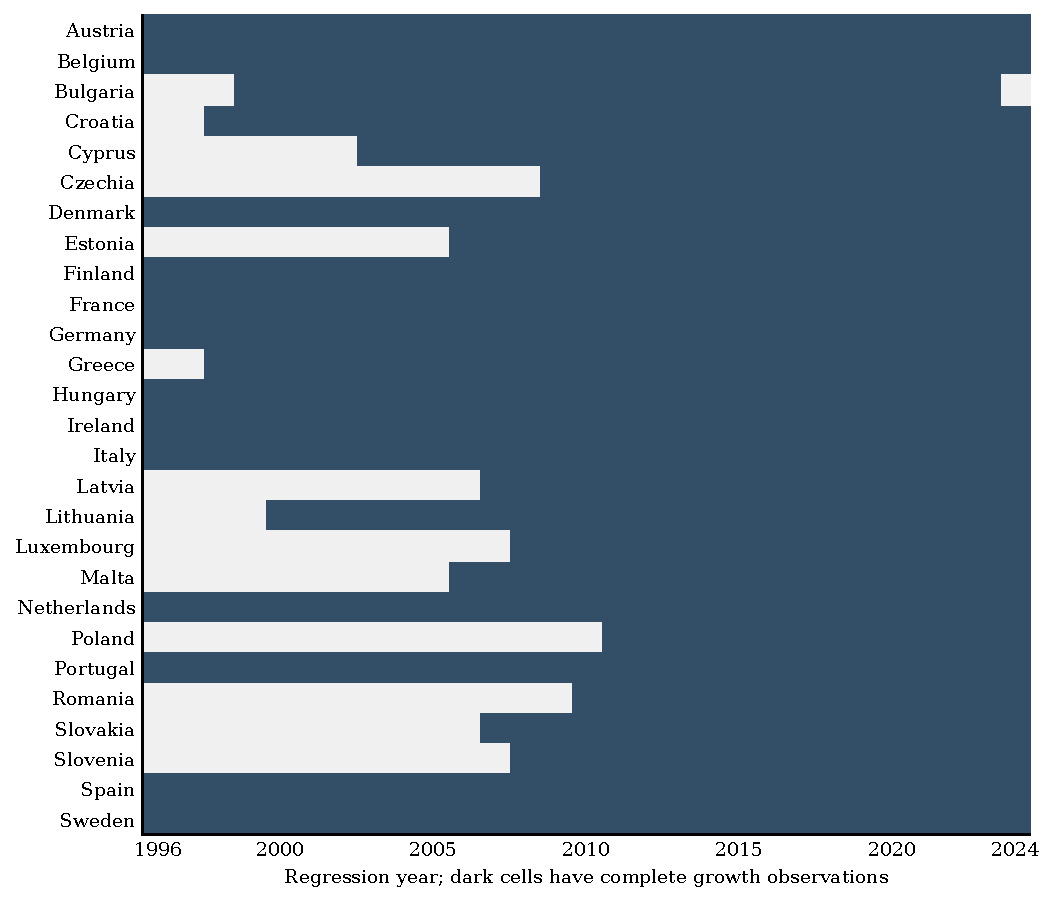
\includegraphics[width=.91\linewidth]{panel/output/coverage.pdf}
\par\vspace{3pt}\begin{minipage}{.91\linewidth}\footnotesize\setstretch{1.08}
Dark cells have observed manufacturing investment, real house-price, and real GDP growth. Blank cells indicate missing growth inputs. The 27-country cohort is fixed throughout the historical window. Source: author calculations from the archived Eurostat and BIS/FRED responses.
\end{minipage}\end{figure}\FloatBarrier

\begin{table}[!htbp]\centering\begin{threeparttable}
\caption{Descriptive statistics for the EU baseline growth sample}\label{tab:2}
\small\setstretch{1.05}\setlength{\tabcolsep}{4pt}\renewcommand{\arraystretch}{1.22}
% Generated by python -m panel.run
\begin{tabularx}{\linewidth}{@{}Y r r r r r@{}}
\toprule
\textbf{Growth series} & \textbf{N} & \textbf{Mean} & \textbf{SD} & \textbf{Min} & \textbf{Max}\\
\midrule
Manufacturing investment & 656 & $2.00$ & $17.18$ & $-87.34$ & $123.02$\\
Real house prices & 656 & $1.93$ & $7.79$ & $-50.46$ & $37.03$\\
Real GDP & 656 & $2.17$ & $3.65$ & $-17.48$ & $22.03$\\
\bottomrule
\end{tabularx}

\begin{tablenotes}[flushleft]\footnotesize\setstretch{1.08}
\item The sample consists of \PanelN{} complete country-year observations over 1996--2024. Growth is 100 times the annual change in natural logarithms. SD is the sample standard deviation. These are pooled descriptive statistics before removing fixed effects. Source: author calculations.
\end{tablenotes}\end{threeparttable}\end{table}\FloatBarrier

Manufacturing investment growth is substantially more dispersed than GDP growth, and both investment and house prices contain large annual movements. The analysis retains these observed values. The alternative outcomes and leave-one-country-out calculations help assess how component composition and individual national histories influence the estimates.

\section{Econometric specification and inference}
The baseline specification includes country effects $\alpha_i$ and year effects $\lambda_t$:
\begin{equation}\label{eq:panel}
g_{it}^{I}=\alpha_i+\lambda_t+\beta g_{it}^{H}+\gamma g_{it}^{Y}+u_{it}.
\end{equation}
Here $I$ denotes manufacturing investment, $H$ real house prices, and $Y$ real GDP. Model 1 omits GDP growth; model 2 is equation~\eqref{eq:panel}; model 3 adds lagged house-price growth:
\begin{equation}\label{eq:lag}
g_{it}^{I}=\alpha_i+\lambda_t+\beta g_{it}^{H}+\phi g_{i,t-1}^{H}+\gamma g_{it}^{Y}+u_{it}.
\end{equation}
The first two models use the same complete-case sample. Country effects absorb stable differences across national manufacturing sectors and property markets, while year effects absorb shocks shared by all countries in a given year. A separate 2020 dummy would be collinear with the year effects and is therefore unnecessary. All specifications are estimated by unweighted OLS with explicit country and year indicators.

Standard errors are clustered by country and by year using the additive multiway estimator of \citet{cameron2011}. The country component permits serial dependence within a country; the year component permits contemporaneous dependence across countries. Each component uses its finite-sample correction, counting all estimated fixed-effect parameters. Two-sided p-values and confidence intervals use a $t$ reference distribution with $\min(G_c,G_t)-1$ degrees of freedom, where $G_c$ and $G_t$ are the observed country and year cluster counts. The baseline has \PanelDof{} reference degrees of freedom. Appendix~\ref{app:inference} gives the covariance formula and verification approach.

GDP is jointly determined with investment and can itself respond to the housing cycle. Conditioning on it changes the question from total co-movement to an association net of national cyclical conditions. Fixed effects do not remove country-specific time-varying credit conditions, exports, energy costs, or industry composition. The slope is therefore interpreted as a conditional short-run association rather than a causal effect or a long-run housing-wealth elasticity. Growth transformations and clustered covariance also leave possible structural breaks as a specification concern.

The sensitivity analysis changes the outcome, country set, period, and covariance convention. Country singletons created by period restrictions are omitted because they supply no within-country variation. Reported sensitivity intervals and p-values are not adjusted for multiple comparisons. The larger observation count broadens geographic evidence, while inference still depends on only 27 country clusters and at most 29 year clusters.

\section{EU panel results}
\subsection{Main specifications}
\begin{table}[!htbp]\centering\begin{threeparttable}
\caption{EU manufacturing investment growth: country and year fixed effects}\label{tab:3}
\small\setstretch{1.05}\setlength{\tabcolsep}{4pt}\renewcommand{\arraystretch}{1.22}
% Generated by python -m panel.run
\begin{tabularx}{\linewidth}{@{}Y r r r@{}}
\toprule
\textbf{Regressor or statistic} & \textbf{1} & \textbf{2} & \textbf{3}\\
\midrule
House price growth & \shortstack{$0.375$\\$(0.202)$} & \shortstack{$0.010$\\$(0.173)$} & \shortstack{$0.113$\\$(0.202)$}\\
GDP growth & \textemdash & \shortstack{$1.894$\\$(0.487)$} & \shortstack{$2.120$\\$(0.540)$}\\
Lagged house price growth & \textemdash & \textemdash & \shortstack{$-0.215$\\$(0.131)$}\\
Observations & 656 & 656 & 629\\
Country clusters & 27 & 27 & 27\\
Year clusters & 29 & 29 & 28\\
Country and year effects & Yes & Yes & Yes\\
Within $R^2$ & $0.022$ & $0.081$ & $0.094$\\
House coefficient p-value & $0.075$ & $0.957$ & $0.581$\\
\bottomrule
\end{tabularx}

\begin{tablenotes}[flushleft]\footnotesize\setstretch{1.08}
\item Country-and-year clustered standard errors are in parentheses. Every model includes country and year effects. Models 1 and 2 share the complete-case baseline sample; model 3 additionally requires lagged house-price growth. Within $R^2$ measures the reduction in residual variation relative to a model containing only the two sets of fixed effects. Source: author calculations.
\end{tablenotes}\end{threeparttable}\end{table}\FloatBarrier

Without national GDP growth, the house-price coefficient is 0.375, with a clustered standard error of 0.202 and p-value of 0.075. Adding GDP growth reduces it to $\PanelBeta$ (standard error $\PanelSE$; p-value $\PanelP$). The baseline interval of $[\PanelLower,\PanelUpper]$ is centered close to zero. Thus the positive co-movement remaining after country and year effects largely disappears when national GDP growth is included.

A ten percentage point increase in house-price log growth corresponds to roughly 0.10 percentage points higher manufacturing investment log growth at the baseline point estimate. The associated interval runs from 3.47 points lower to 3.66 points higher. The GDP coefficient is 1.894, while the within $R^2$ is $\PanelWithin$. These estimates describe variation remaining after the country and year means have been accounted for.

In model 3, contemporaneous house-price growth has a coefficient of 0.113 and its lag has a coefficient of $-0.215$. Their individual p-values are 0.581 and 0.111. The lagged specification uses 629 observations, compared with \PanelN{} in the baseline. This extension leaves the evidence for a common negative manufacturing-investment relationship weak.

\subsection{Components, windows, and sample balance}
\begin{table}[!htbp]\centering\begin{threeparttable}
\caption{Sensitivity of the EU house-price coefficient}\label{tab:4}
\small\setstretch{1.05}\setlength{\tabcolsep}{3pt}\renewcommand{\arraystretch}{1.25}
% Generated by python -m panel.run
\begin{tabularx}{\linewidth}{@{}Y r r r r r@{}}
\toprule
\textbf{Specification} & \textbf{N} & \textbf{Countries} & \textbf{Estimate} & \textbf{95 percent CI} & \textbf{p-value}\\
\midrule
Equipment investment & 652 & 27 & $0.060$ & $[-0.363, 0.484]$ & $0.772$\\
Intellectual property & 652 & 27 & $-0.326$ & $[-0.626, -0.026]$ & $0.034$\\
Exclude Spain & 627 & 26 & $0.009$ & $[-0.349, 0.368]$ & $0.958$\\
1996--2007 & 202 & 20 & $-0.200$ & $[-0.526, 0.126]$ & $0.204$\\
2008--2024 & 452 & 27 & $0.142$ & $[-0.430, 0.714]$ & $0.607$\\
Exclude 2020 and 2021 & 602 & 27 & $-0.144$ & $[-0.485, 0.197]$ & $0.393$\\
End in 2023 & 630 & 27 & $0.048$ & $[-0.307, 0.402]$ & $0.785$\\
Balanced 2010--2024 & 375 & 25 & $-0.171$ & $[-0.575, 0.234]$ & $0.381$\\
Country clustering only & 656 & 27 & $0.010$ & $[-0.173, 0.192]$ & $0.916$\\
\bottomrule
\end{tabularx}

\begin{tablenotes}[flushleft]\footnotesize\setstretch{1.08}
\item Each row modifies model 2. Equipment and intellectual property replace the outcome. The balanced window requires all 15 annual growth observations during 2010--2024 and retains 25 countries. Country and year effects remain in every row; only the last row changes clustering to country alone. Intervals use the reference degrees of freedom described in Section~5. Source: author calculations.
\end{tablenotes}\end{threeparttable}\end{table}\FloatBarrier

The equipment coefficient is 0.060, with an interval of $[-0.363,0.484]$. Intellectual property investment has a coefficient of $-0.326$, with an interval of $[-0.626,-0.026]$ and unadjusted p-value of 0.034. The latter is the most distinct component result, but it is one of several sensitivity estimates. It motivates closer study of investment composition rather than a conclusion about the total manufacturing response.

The pre-2008 sample gives $-0.200$, while the 2008--2024 sample gives 0.142. Both intervals include zero. Excluding 2020 and 2021 produces $-0.144$, and ending the sample in 2023 produces 0.048. The balanced 2010--2024 estimate is $-0.171$ with an interval of $[-0.575,0.234]$. The aggregate conclusion therefore does not rely on one particular window or on using the longest possible unbalanced sample.

\begin{figure}[!htbp]\centering
\caption{EU baseline and sensitivity estimates}\label{fig:coefficients}
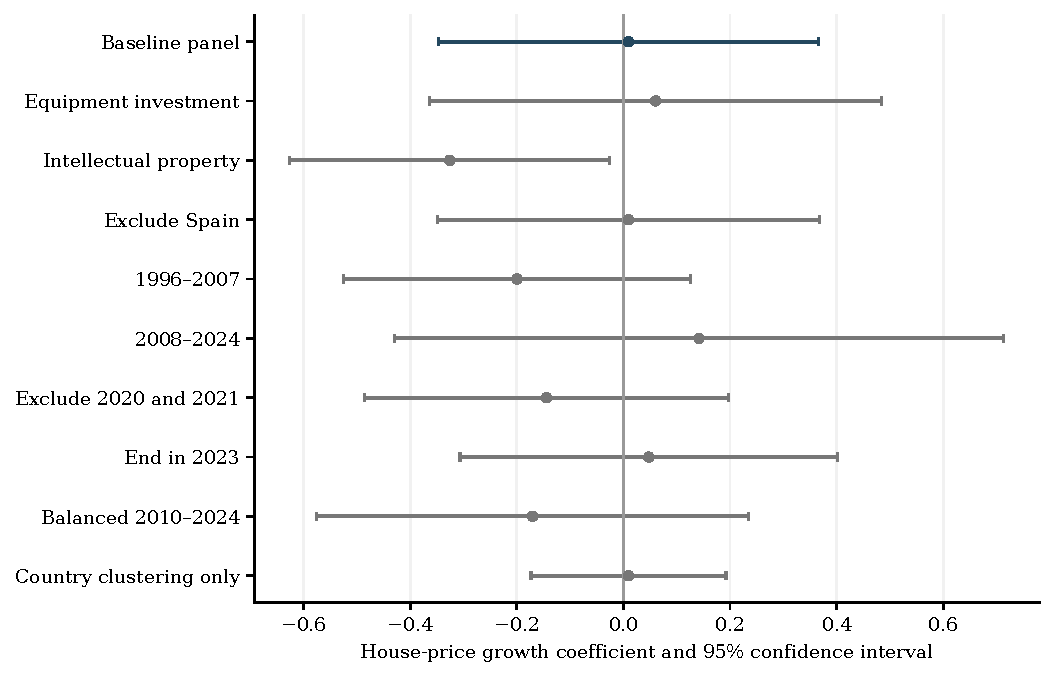
\includegraphics[width=.95\linewidth]{panel/output/coefficients.pdf}
\par\vspace{3pt}\begin{minipage}{.95\linewidth}\footnotesize\setstretch{1.08}
Points show the house-price growth coefficient; bars show 95 percent intervals. All rows include GDP growth and country and year effects. Covariance is clustered by both dimensions except in the final row. Source: author calculations.
\end{minipage}\end{figure}\FloatBarrier

\subsection{Country influence and inference}
Removing Spain yields 0.009, almost identical to the baseline. Across all 27 leave-one-country-out fits, the point estimate ranges from $\PanelLooMin$ to $\PanelLooMax$. This stability around zero indicates that no single national history generates the baseline conditional estimate.

The country-only clustered standard error is 0.089, compared with 0.173 under country-and-year clustering. Accounting for dependence across countries within a year therefore matters for the reported uncertainty. The two-way estimate is used throughout the main results rather than selecting the covariance convention that gives a narrower interval.

\section{Spain as the institutional case study}
\subsection{National patterns during the boom}
\begin{figure}[!htbp]\centering
\caption{House prices and manufacturing investment in Spain}\label{fig:spain}
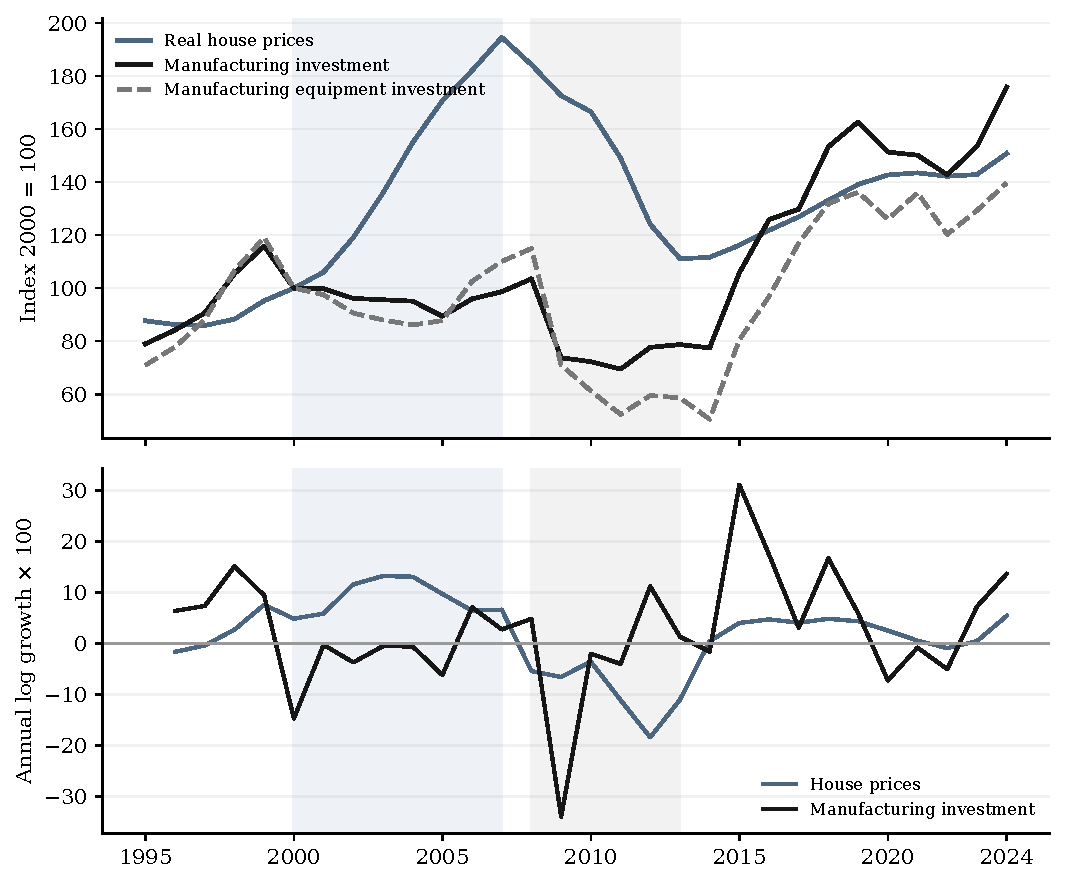
\includegraphics[width=.94\linewidth]{figures/figure1.pdf}
\par\vspace{3pt}\begin{minipage}{.94\linewidth}\footnotesize\setstretch{1.08}
The upper panel rebases each series to 2000 = 100; the lower panel shows annual log growth multiplied by 100. Shading marks 2000--2007 and 2008--2013. Sources: Eurostat and national sources, BIS Residential Property Price database via FRED, using the archived Spain sample.
\end{minipage}\end{figure}\FloatBarrier

Between 2000 and 2007, annual average real house prices in Spain rose by 94.6 percent, while real manufacturing GFCF declined by 1.4 percent. Equipment investment rose by 10.1 percent and intellectual property investment by 85.1 percent. These endpoint changes show the importance of composition within manufacturing investment. Investment log growth averaged $-1.49$ percentage points in 2001--2003 and 0.78 in 2004--2007, while house-price growth averaged 10.22 and 8.97.

\subsection{National regression benchmarks}
\begin{table}[!htbp]\centering\begin{threeparttable}
\caption{Spain: national time-series benchmarks}\label{tab:spain}
\small\setstretch{1.05}\setlength{\tabcolsep}{4pt}\renewcommand{\arraystretch}{1.22}
% Generated by replication/render_tables.py; edit the code or layout template.
\begin{tabularx}{\linewidth}{@{}>{\hsize=2.10\hsize\linewidth=\hsize}Y >{\hsize=.725\hsize\linewidth=\hsize}C >{\hsize=.725\hsize\linewidth=\hsize}C >{\hsize=.725\hsize\linewidth=\hsize}C >{\hsize=.725\hsize\linewidth=\hsize}C @{}}
\toprule
\textbf{Regressor or statistic} & \textbf{1} & \textbf{2} & \textbf{3} & \textbf{4}\\
\midrule
House price growth & \shortstack{$0.161$\\$(0.300)$} & \shortstack{$-0.076$\\$(0.256)$} & \shortstack{$-0.263$\\$(0.434)$} & \shortstack{$0.045$\\$(0.581)$}\\
GDP growth & \textemdash & \shortstack{$1.105$\\$(0.721)$} & \shortstack{$1.942$\\$(2.139)$} & \shortstack{$2.023$\\$(2.152)$}\\
2020 indicator & \textemdash & \textemdash & \shortstack{$17.123$\\$(30.272)$} & \shortstack{$19.271$\\$(30.302)$}\\
Lagged house price growth & \textemdash & \textemdash & \textemdash & \shortstack{$-0.403$\\$(0.327)$}\\
Constant & \shortstack{$2.459$\\$(2.495)$} & \shortstack{$0.703$\\$(2.773)$} & \shortstack{$-1.203$\\$(5.157)$} & \shortstack{$-1.428$\\$(5.172)$}\\
Observations & $29$ & $29$ & $29$ & $28$\\
$R^2$ & $0.010$ & $0.102$ & $0.125$ & $0.146$\\
House coefficient p-value & $0.596$ & $0.769$ & $0.551$ & $0.940$\\
\bottomrule
\end{tabularx}

\begin{tablenotes}[flushleft]\footnotesize\setstretch{1.08}
\item These are the archived Spain models. Models 1--3 use 1996--2024; model 4 adds lagged house-price growth and uses 1997--2024. Parentheses contain Newey--West standard errors with one annual lag and the $n/(n-k)$ correction. The columns are separate national specifications, not the EU models. Source: author calculations.
\end{tablenotes}\end{threeparttable}\end{table}\FloatBarrier

The Spain model controlling for GDP growth and a 2020 indicator gives a house-price coefficient of $-0.263$, with an interval of $[-1.157,0.632]$. For 1996--2007, the coefficient is $-0.746$ with an interval of $[-1.287,-0.205]$; restricting the window to 2001--2007 instead gives $-0.231$ with an interval of $[-2.080,1.619]$. The longer pre-2008 window combines the investment expansion of the late 1990s with subsequent years. These national patterns explain why Spain merits closer institutional study, while the EU estimates provide the broader comparison.

\section{Microeconomic evidence and a design for causal analysis}

\subsection{What the published estimates establish}

\begin{table}[!htbp]
\centering
\begin{threeparttable}
\caption{Selected estimates from the Spanish microdata literature}
\label{tab:5}
\small\setstretch{1.05}
\setlength{\tabcolsep}{4pt}
\renewcommand{\arraystretch}{1.25}
\begin{tabularx}{\linewidth}{@{}>{\hsize=1.65\hsize\linewidth=\hsize}Y >{\hsize=.675\hsize\linewidth=\hsize}C >{\hsize=.675\hsize\linewidth=\hsize}C@{}}
\toprule
\textbf{Outcome} & \textbf{2001--2003} & \textbf{2004--2007}\\
\midrule
Loan level non-housing credit growth & $-2.29 (0.92)$ & $4.82 (1.09)$\\
Firm level credit growth all firms & $-2.89 (0.96)$ & $3.34 (1.53)$\\
Firm value added growth & $-0.38 (0.15)$ & $0.94 (0.53)$\\
Firm investment growth & $-0.32 (0.18)$ & $1.89 (0.97)$\\
\bottomrule
\end{tabularx}
\begin{tablenotes}[flushleft]
\footnotesize\setstretch{1.08}
\item Source: \citet*{martin2021}, published Tables 1, 3, and 4. Entries are effects of a one-standard-deviation increase in bank or firm exposure; clustered standard errors are in parentheses. Credit growth is the cumulative percentage change between the endpoints of each interval, rather than annual log growth. Their firm investment measure is based on changes in the book value of fixed assets and differs from national accounts GFCF. These estimates are reported from the source, not re-estimated here.
\end{tablenotes}
\end{threeparttable}
\end{table}
\FloatBarrier

The loan level estimates contrast banks lending to the same firm, helping to hold borrower demand fixed. The firm level results address whether a borrower can compensate by obtaining credit elsewhere. The investment estimates are less precise than the credit results. This pattern supports a financial transmission mechanism, while leaving uncertainty about the size of the real investment response. It also explains why a national manufacturing regression need not recover the bank exposure coefficients.


Aggregate counterfactuals answer an additional question. In the calibrated model of \citeauthor{martin2021}, non-housing credit is 7.7 percent below a counterfactual without financial transmission in 2004 and 1.8 percent above it in 2008. Those figures depend on the model and its calibration; they are not direct time series regression coefficients. Closing a credit gap by 2008 does not establish the absence of subsequent crisis costs or the recovery of every forgone investment project.


\subsection{Loan and firm level specifications}

A causal extension requires matched bank--firm lending and firm accounts, with authorization to use the underlying restricted data. Bank exposure $E_b$ can be defined as housing loans divided by total loans in a fixed baseline year, and standardized before estimation. In a panel of firms borrowing from multiple banks, a candidate specification is


\begin{equation}\label{eq:7}
\begin{aligned}\Delta\ln L_{ibt}={}&\mu_{it}+\eta_{ib}+\sum_{\tau\neq\tau_0}\beta_\tau E_b\mathbf{1}\{t=\tau\}\\&+X_{b0}^{\top}\Gamma_t+\varepsilon_{ibt}.\end{aligned}
\end{equation}

Here $i$ indexes firms, $b$ banks, and $t$ calendar years. The sum in equation~\eqref{eq:7} omits the reference year $\tau_0$, which can be set to the baseline year 2000. Firm-by-year effects $\mu_{it}$ absorb demand shocks common to a firm's lenders, following the logic of \citet{khwaja2008}. Relationship effects $\eta_{ib}$ absorb stable bank--firm matching. Baseline bank controls interacted with time can address observable differences in capital, liquidity, size, and lender type. Standard errors should allow dependence within banks and firms. Identification still requires that exposure is unrelated to omitted changes in bank credit supply after conditioning on these terms. The baseline year 2000 predates much of the boom but is not an untreated random assignment.


A firm-level extension can relate investment to the loan-weighted baseline exposure of its lenders, using firm effects and location-by-industry-by-year effects. This evaluates whether bank shocks survive credit substitution. However, it requires additional assumptions about lender matching and borrower investment opportunities. Results for multi-bank firms also need not generalize to firms with a single lender. Exits, lender switching, bank mergers, and zero or newly created loans must be handled explicitly rather than silently dropped by a logarithmic transformation.


\subsection{Collateral and allocation}

A separate design should interact local house price growth with a firm's baseline property holdings. Firm effects and municipality-by-year effects can absorb stable heterogeneity and common local shocks while leaving interactions with baseline firm characteristics identified. If local house price growth is instrumented using pre-boom land supply interacted with aggregate mortgage rate changes, each endogenous interaction requires a corresponding instrument. The national rate shock must not have differential direct effects on firm investment correlated with land supply, conditional on the controls.


That exclusion restriction is demanding because land scarcity can also affect industrial premises, local development, and firm location. A credible implementation should report the relevant first-stage diagnostics, examine pre-trends, use inference at the geographic level of the instrument, and allow for few effective aggregate shocks. Measuring misallocation additionally requires estimated marginal returns, productivity, or project outcomes. A large response among property owners alone can also reflect the relaxation of previously inefficient financing constraints. These firm-level outcomes would connect the collateral response to its productivity consequences.



\section{Discussion}
The panel and the Spanish microeconomic evidence describe different margins. Across European country-years, house-price growth has little conditional association with total manufacturing investment growth once national GDP growth and common annual conditions are included. Within Spain, lender exposure and collateral ownership help explain which firms receive credit and how the response evolves during a housing boom. Reallocation across borrowers and investment components can coexist with a small aggregate coefficient.

The panel addresses the original study's narrow geographic base, but several measurement and specification issues remain. National house prices may not match the location or type of property pledged by manufacturing firms. GFCF records expenditure rather than its financing source or return. Coverage is uneven, national accounts are revised, and common slope coefficients can conceal institutional heterogeneity. The balanced sample and country-influence checks reduce dependence on particular histories without replacing firm-level information.

For policy, the relevant distinction is between expanding finance for productive but constrained firms and directing funds toward borrowers with valuable property but lower-return projects. Capital and concentration measures address risks in bank portfolios; information about cash flows and investment opportunities may reduce reliance on property collateral. The near-zero aggregate panel estimate does not make those distributional questions disappear. They require evidence about borrowers, lenders, and project outcomes.

\section{Conclusion}
An EU country-by-year panel substantially broadens the evidence on house prices and manufacturing investment. The baseline uses \PanelN{} observations from all 27 current member countries, with country and year fixed effects and clustering along both dimensions. Its house-price coefficient is $\PanelBeta$ after including GDP growth, with an interval of $[\PanelLower,\PanelUpper]$. Alternative windows, a balanced sample, and country exclusions leave the total-investment estimates imprecise. Intellectual property investment provides a narrower negative component result that warrants further investigation.

Spain remains informative because published microdata studies identify credit-supply and collateral mechanisms that national aggregates combine. The broader evidence supports an institution- and composition-sensitive account of housing finance rather than a uniform European crowding-out effect. Future work linking the panel to bank exposure, firm property holdings, and investment returns could explain how the national patterns emerge from individual financing decisions.

\clearpage
\phantomsection\addcontentsline{toc}{section}{References}
\bibliographystyle{plainnat}\bibliography{references}
\clearpage\appendix
\renewcommand{\theequation}{\thesection.\arabic{equation}}\setcounter{equation}{0}
\section{Country coverage}\label{app:coverage}
\begin{table}[!htbp]\centering\begin{threeparttable}
\caption{Complete-case baseline observations by country}\label{tab:coverage}
\small\setstretch{1.0}\setlength{\tabcolsep}{4pt}\renewcommand{\arraystretch}{1.12}
% Generated by python -m panel.run
\begin{tabularx}{\linewidth}{@{}Y r r r@{}}
\toprule
\textbf{Country} & \textbf{First year} & \textbf{Last year} & \textbf{N}\\
\midrule
Austria (AT) & 1996 & 2024 & 29\\
Belgium (BE) & 1996 & 2024 & 29\\
Bulgaria (BG) & 1999 & 2023 & 25\\
Croatia (HR) & 1998 & 2024 & 27\\
Cyprus (CY) & 2003 & 2024 & 22\\
Czechia (CZ) & 2009 & 2024 & 16\\
Denmark (DK) & 1996 & 2024 & 29\\
Estonia (EE) & 2006 & 2024 & 19\\
Finland (FI) & 1996 & 2024 & 29\\
France (FR) & 1996 & 2024 & 29\\
Germany (DE) & 1996 & 2024 & 29\\
Greece (EL) & 1998 & 2024 & 27\\
Hungary (HU) & 1996 & 2024 & 29\\
Ireland (IE) & 1996 & 2024 & 29\\
Italy (IT) & 1996 & 2024 & 29\\
Latvia (LV) & 2007 & 2024 & 18\\
Lithuania (LT) & 2000 & 2024 & 25\\
Luxembourg (LU) & 2008 & 2024 & 17\\
Malta (MT) & 2006 & 2024 & 19\\
Netherlands (NL) & 1996 & 2024 & 29\\
Poland (PL) & 2011 & 2024 & 14\\
Portugal (PT) & 1996 & 2024 & 29\\
Romania (RO) & 2010 & 2024 & 15\\
Slovakia (SK) & 2007 & 2024 & 18\\
Slovenia (SI) & 2008 & 2024 & 17\\
Spain (ES) & 1996 & 2024 & 29\\
Sweden (SE) & 1996 & 2024 & 29\\
\bottomrule
\end{tabularx}

\begin{tablenotes}[flushleft]\footnotesize\setstretch{1.08}
\item Each observation requires consecutive-year positive levels for manufacturing investment, real house prices, and GDP. The cohort comprises all current EU27 members. A country-year CSV records exact omitted years and source status flags; the first and last years shown here summarize usable growth coverage. Source: author calculations.
\end{tablenotes}\end{threeparttable}\end{table}\FloatBarrier

\clearpage
\section{Covariance implementation and verification}\label{app:inference}
\subsection{Country-and-year clustering}
Let $\mathbf s_{it}=\mathbf x_{it}\widehat u_{it}$ denote a score contribution from the full dummy-variable design, including the country and year effects. Country and year score totals are $\mathbf S_i=\sum_t\mathbf s_{it}$ and $\mathbf S_t=\sum_i\mathbf s_{it}$. The reported covariance is
\begin{equation}\label{eq:cluster}
\widehat{\mathbf V}=(\mathbf X^{\top}\mathbf X)^{-1}
\left[c_c\sum_i\mathbf S_i\mathbf S_i^{\top}
+c_t\sum_t\mathbf S_t\mathbf S_t^{\top}
-c_{ct}\sum_{i,t}\mathbf s_{it}\mathbf s_{it}^{\top}\right]
(\mathbf X^{\top}\mathbf X)^{-1}.
\end{equation}
For component $d$, $c_d=G_d/(G_d-1)\,(N-1)/(N-K)$. Here $K$ is the rank of the full estimated design, including fixed effects. Each observed country-year cell is unique, so the intersection component has $G_{ct}=N$. The estimator follows \citet{cameron2011}; the main code calls \texttt{statsmodels}' two-group covariance routine.

An independent implementation aggregates the three sets of scores and reproduces each reported covariance. Alternating country/year projections separately recover the full dummy-variable slopes; iteration handles the unbalanced panel. Both checks cover all 12 specifications.

\subsection{Calendar gaps in the Spain benchmarks}
The Spain benchmarks use the Bartlett-kernel covariance of \citet{newey1987}, pairing observations at their actual calendar-year distances. Omitting 2020 does not make 2019 and 2021 adjacent under a one-year bandwidth.

Let $\mathcal T$ denote the set of included calendar years and let
$\mathbf s_t=\mathbf x_t\widehat u_t$ be the score contribution for year $t$.
The Newey--West covariance matrix is
\begin{equation}\label{eq:hac}
\widehat{\operatorname{Var}}(\widehat{\bm\beta})
=\frac{n}{n-k}(\mathbf X^{\top}\mathbf X)^{-1}\widehat{\mathbf S}_L(\mathbf X^{\top}\mathbf X)^{-1},
\end{equation}
where
\begin{equation}\label{eq:meat}
\begin{aligned}
\widehat{\mathbf S}_L={}&\sum_{t\in\mathcal T}\mathbf s_t\mathbf s_t^{\top}\\
&+\sum_{h=1}^{L}\left(1-\frac{h}{L+1}\right)
\sum_{\substack{t,s\in\mathcal T\\t-s=h}}
\left(\mathbf s_t\mathbf s_s^{\top}+\mathbf s_s\mathbf s_t^{\top}\right).
\end{aligned}
\end{equation}
Here $n$ is the number of included observations, $k$ includes the intercept, and $L$ is
the annual bandwidth. Cross-products use actual calendar distances when years are
omitted. Confidence intervals use the $t$ critical value with $n-k$ degrees of freedom.

The function \texttt{calendar\_hac\_meat} matches observations by year distance. The independent \texttt{statsmodels} check pads omitted years with zero scores; OLS and the finite-sample factor continue to use the observed sample size.


\end{document}
